\documentclass{book}
\usepackage{listings}
\usepackage{hyperref}
\usepackage{verbatim}
\usepackage{amsmath}
\usepackage[backend=bibtex, sorting=none, style=numeric-comp, defernumbers]{biblatex}
\usepackage{graphicx}
\usepackage{subcaption}
\UseRawInputEncoding
\captionsetup{compatibility=false}

\addbibresource{\jobname.bib}

\begin{document}
\title{Chapter 6 - Computer Vision}
\author {Joydeep Bhattacharjee}

\maketitle

% https://cetra3.github.io/blog/face-detection-with-tensorflow-rust/
% https://docs.rs/aperature/0.1.1/aperature/
% git@github.com:atomashpolskiy/rustface.git

In the last chapter, we took at look at how machine learning applies in the domain of human languages. That covers our senses of speech and sound. Another sense where machine learning has a huge influence is our sense of vision and how machine learning is able to capture the essence of images. The overall branch is termed computer vision and there has been great strides in solving computer vision problems in Rust as we will see in this chapter.

As part of this chapter we will look at different application in computer vision such as:

\begin{itemize}
	\item Image classification
	\item Using pretrained models
	\item Neural style transfer
	\item Face detection
\end{itemize}

\section{Image Classification}%
Image classification is the application of machine learning to images, where the objective is given an image and a model trained on finding objects of interest, the model would identify if the object is present in the image or not. This is achieved by defining a set of target classes (objects to identify in images), a model is trained to  identify them using labeled example photos.

Image classification using traditional models was achieved by adding new features from pixel data, such as color histograms, textures and shapes. The downside of this approach was that feature engineering in the case of image classification was a huge cost. Features needed to be tuned quite precisely and hence building robust models was very challenging with low accuracy in many cases.

\subsection{Convolutional Neural Networks}%
In contrast with the traditional models Neural networks with convolutional layers was seen to have better results for the image classification tasks. A CNN progressively extract higher and higher level representations of the image content. Instead of preprocessing the data to derive features like textures and shapes, a CNN takes just the raw pixels of the image as input and "learns" how to extract those features, and ultimately infer what object they constitute.

% https://developers.google.com/machine-learning/practica/image-classification/convolutional-neural-networks
\label{sub:Convolutional Neural Networks}
The CNN starts with an input feature map of three dimensions where the size of the first two dimensions is the length and width of the images in pixels. The size of the third dimension is the number of channels in the image and is generally 3. The CNN comprises of stacks of modules, where each module performs three operations.

\begin{enumerate}
	\item Convolution layer, where tiles of the input feature map are extracted and filters are applied to the features. A filter matrix is slided over the feature matrix and sum of the element wise multiplication is stored in the resulting matrix. During training the CNN "learns" the optimal value for the feature matrix, that enable it to extract meaningful features.
		\begin{figure}[h!]
                  \centering
                  \begin{subfigure}[b]{0.4\linewidth}
                    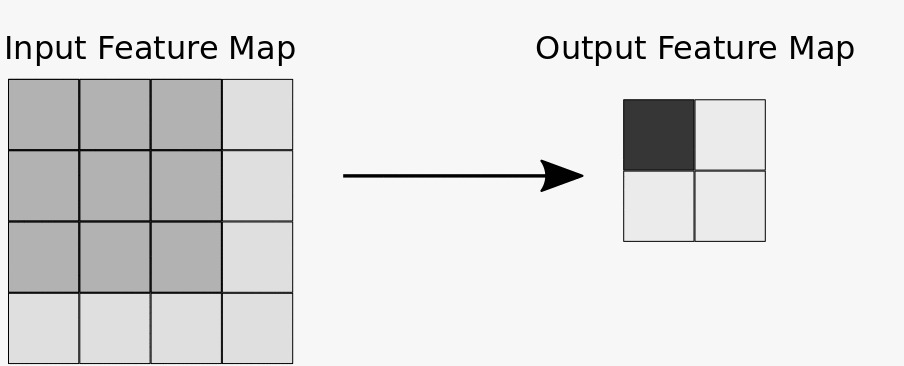
\includegraphics[width=\linewidth]{Figures/cnn1.jpg}
                    \caption{1.}
                  \end{subfigure}
                  \begin{subfigure}[b]{0.4\linewidth}
                    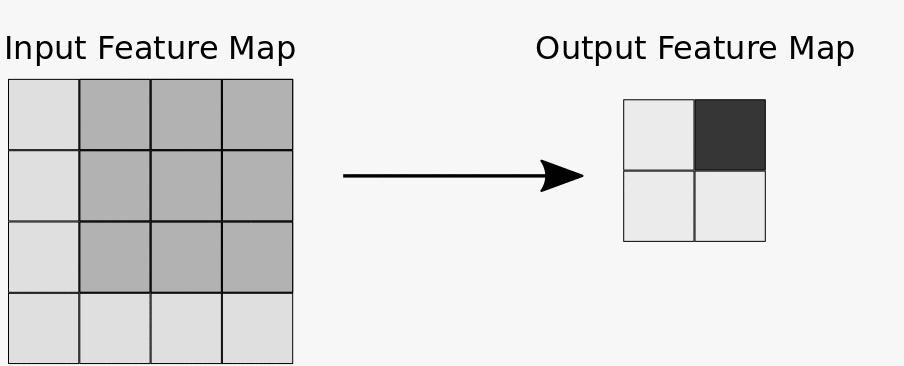
\includegraphics[width=\linewidth]{Figures/cnn2.jpg}
                    \caption{2.}
                  \end{subfigure}
                  \begin{subfigure}[b]{0.4\linewidth}
                    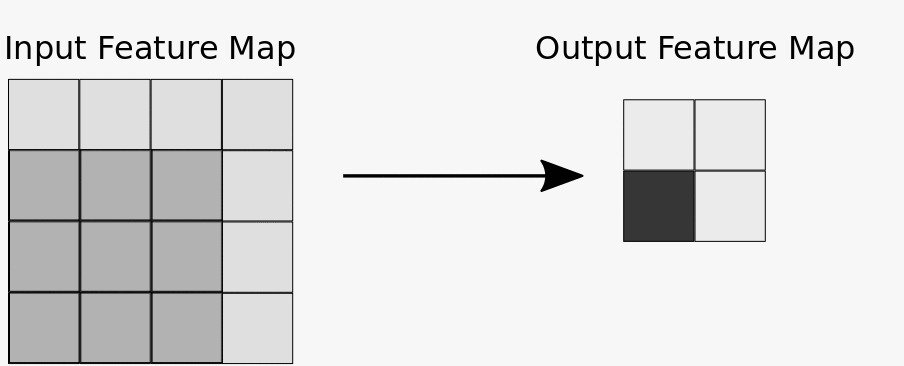
\includegraphics[width=\linewidth]{Figures/cnn3.jpg}
                    \caption{3.}
                  \end{subfigure}
                  \begin{subfigure}[b]{0.4\linewidth}
                    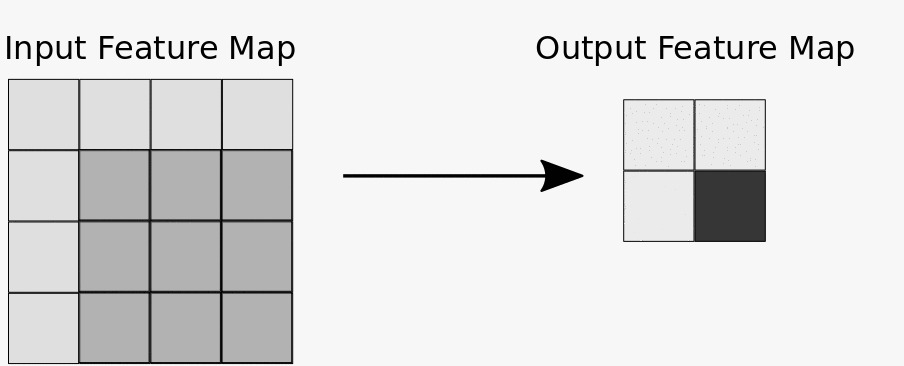
\includegraphics[width=\linewidth]{Figures/cnn4.jpg}
                    \caption{4.}
                  \end{subfigure}
                  \caption{Extracting features through convolution.}
                  \label{fig:coffee}
                \end{figure}
	\item A Relu layer is introduced after the convolution layer in order to introduce non linearity into the model. The Relu function is defined as $f(x)=max(0,x)$ and is given by the below figure1.
		\begin{figure}
		\begin{center}
			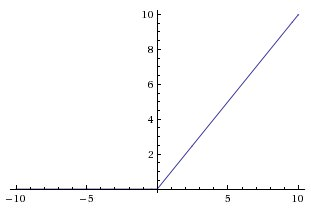
\includegraphics[scale=0.5]{Figures/relu.jpg}
		\end{center}
		\caption{Relu function}
		\label{fig:relu}
		\end{figure}
	\item After application of the Relu activation function, pooling is applied to downsample the convolved feature. Downsampling needs to be done by keeping the most critical feature information while at the same time reducing the dimensions as much as possible. Generally max pooling is used where tiles are extracted from the feature map and the maximum value is kept from each tile while discarding all the other values.
\end{enumerate}

At the end of the CNN layer, a one or more layers of fully connected layers are needed to perform the classification based on the features extracted by the convolutions.

\subsection{Rust and Torch}%
As seen in chapter2, we can use the torch deeplearning library\footnote{\href{}{https://pytorch.org/}}, which many developers know as pytorch. Since in the case of computer vision deep learning has been shown to have the best results, we will be focusing mostly on creating and using deep neural models. Currently torch is the most usable in terms of creating and using deep neural models in Rust and hence in this chapter, we will mostly be working in the torch paradigm.
\label{sub:rust_and_torch}

\subsection{Torch Dataset}%
To build an image classification model, we will be using the Caltech101\footnote{\href{}{http://www.vision.caltech.edu/Image\_Datasets/Caltech101/}} data set. To download the files, go to the link that is given in the footnote and download the images.

\begin{lstlisting}[caption={download images}, basicstyle=\tiny]
$ wget http://www.vision.caltech.edu/Image_Datasets/Caltech101/101_ObjectCategories.tar.gz
$ gunzip -c 101_ObjectCategories.tar.gz | tar xvf -
\end{lstlisting}

or you can download using the browser. If download using the browser you would still need to uncompress it using the command above.

\begin{figure}[htpb]
	\centering
	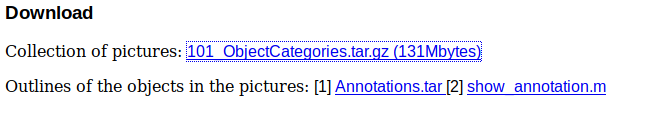
\includegraphics[width=0.8\linewidth]{Figures/downloadcaltech101.png}
	\caption{Download caltech101}
	\label{fig:Figures/downloadcaltech101}
\end{figure}

Similar to \lstinline{torch-vision}, to work with image datasets we have the \lstinline{vision::Dataset} structure. Lets take a look at this structure.

\begin{lstlisting}[caption={tch-rs/src/vision/dataset.rs}, basicstyle=\small]
#[derive(Debug)]
pub struct Dataset {
  pub train_images: Tensor,
  pub train_labels: Tensor,
  pub test_images: Tensor,
  pub test_labels: Tensor,
  pub labels: i64,
}
\end{lstlisting}

A handy function in the \lstinline{tch} crate to load the images and convert it to the \lstinline{Dataset} mentioned above is through using the function \lstinline{tch::vision::imagenet::load_from_dir}. To do that we will need to separate the caltech101 files that we have created into training and val folders in the below format. Inside the root folder, we need to have two folders "train" and "val" and inside those folders we need to have the different images inside the folders with folder names as the labels. Or in other words all images with the same label would be in the same folder.

\begin{lstlisting}[caption={}, basicstyle=\tiny]
dataset
├── train
│   ├── accordion
│   │   ├── image_0001.jpg
│   │   ├── image_0002.jpg
│   ├── airplanes
│   │   ├── image_0001.jpg
│       └── image_0060.jpg
	...
└── val
    ├── accordion
    │   └── image_0036.jpg
    ├── airplanes
    │   └── image_0685.jpg
	...
\end{lstlisting}

The caltech dataset when uncompressed is in this format.

\begin{lstlisting}[caption={}, basicstyle=\tiny]
101_ObjectCategories
├── accordion
│   ├── image_0001.jpg
│   ├── image_0002.jpg
├── airplanes
│   ├── image_0001.jpg
│   ├── image_0002.jpg
    ...

102 directories, 9145 files
\end{lstlisting}

Although the directory structure is mostly similar still we will need to write a small function that will split the dataset into train and validation sets. The below function that is written for this purpose is a recursive function where if path is a directory then we will go deeper else we will run the testing function on one file and training function on the other files. The variable \lstinline{this_label} is there to check if the testing function has already been run on the current label. We will implement the \lstinline{train_fn} and \lstinline{test_fn} as functions that implement the actual movement. This could have been implemented here but implementing this as separate functions will make this more modular and easily testable.

\begin{lstlisting}[caption={chapter6/pytorch-image-classification/src/main.rs}, basicstyle=\small]
use std::io;
use std::fs::{self, DirEntry, copy, create_dir_all};
use std::path::Path;

fn visit_dir(dir: &Path,
             train_fn: &Fn(&DirEntry),
	     test_fn: &Fn(&DirEntry)) -> io::Result<()> {
  if dir.is_dir() {
    let mut this_label = String::from("");
    for entry in fs::read_dir(dir)? {
      let entry = entry?;
      let path = entry.path();
      if path.is_dir() {
        visit_dir(&path, train_fn, test_fn)?;
      } else {
        let full_path: Vec<String> = path.to_str().unwrap()
	  .split("/").into_iter()
          .map(|x| x[..].to_string()).collect();
        if this_label == full_path[1] {
          train_fn(&entry); // move the training file
        } else {
          test_fn(&entry); // move the testing file
        }
	// the second entry is the label
	this_label = full_path[1].clone();
      }
    }
  }
  Ok(())
}
\end{lstlisting}

Now we will need to define the actual file copying function from source folder to destination folder. Remember that our destination path should be in the format "\lstinline{root_dataset_foldername} > 'train' or 'val' folder based on if the file is a training file or a validation file > label as folder name for the particular image > image file". The function should create all the intermediate directories in case they are not present. This can be implemented using the \lstinline{move_file} function below.

\begin{lstlisting}[caption={chapter6/pytorch-image-classification/src/main.rs}, basicstyle=\small]
use std::fs::{self, direntry, copy, create_dir_all};
const dataset_folder: &str = "dataset";
fn move_file(from_path: &direntry, to_path: &path) -> io::result<()> {
  let root_folder = path::new(dataset_folder);
  let second_order = root_folder.join(to_path);
  let full_path: vec<string> = from_path.path().to_str().unwrap()
    .split("/").into_iter().map(|x| x[..].to_string()).collect();
  let label = full_path[1].clone();
  let third_order = second_order.join(label);
  create_dir_all(&third_order)?;
  let filename = from_path.file_name();
  let to_filename = third_order.join(&filename);
  copy(from_path.path(), to_filename)?;
  ok(())
}
\end{lstlisting}

As we can see above, root folder is the dataset folder, \lstinline{to_path} is essentially if the file needs to go to the train folder or the validation folder. Next we will split the source path to the \lstinline{full_path} variable so that we are able to retrieve the label from the full path. Once all the paths are joined the function \lstinline{create_dir_all} from \lstinline{std::fs} standard library is used to create all the directories. The respective file name is parsed from the \lstinline{from_path} variable, joined to the \lstinline{to_filename} variable. Once we have successfully constructed the full path for the destination path we pass the destination path, in other words the \lstinline{to_filename} variable to the \lstinline{copy} function from \lstinline{std::fs} standard  library to create the folder structure.

We should now be able to run this code and segregate the data set to train and val images.

\begin{lstlisting}[caption={chapter6/pytorch-image-classification/src/main.rs}, basicstyle=\small]
fn main() -> failure::Fallible<()> {
  let obj_categories = Path::new("101_ObjectCategories");
  let move_to_train = |x: &DirEntry| {
    let to_folder = Path::new("train");
    move_file(&x, &to_folder).unwrap();
  };
  let move_to_test =
    |x: &DirEntry| {
      let to_folder = Path::new("val");
      move_file(&x, &to_folder).unwrap();
    };
    visit_dir(
      &obj_categories, &move_to_train,
      &move_to_test).unwrap();
    println!(
      "files kept in the imagenet format in {}", DATASET_FOLDER);
  ... remaining code
\end{lstlisting}

In the above code we create two closures, \lstinline{move_to_train} and \lstinline{move_to_test} that will pass to \lstinline{move_file} function the appropriate destination folder. These closures are then passed to the \lstinline{visit_dir} function that will run them as we had already seen. Running the code till now should segregate the folders and arrange them in the imagenet format. We should now be able to use the \lstinline{load_from_dir} function which is a handy function in \lstinline{torch::vision}.

\begin{lstlisting}[caption={chapter6/pytorch-image-classification/src/main.rs}, basicstyle=\small]
use tch::vision::imagenet::load_from_dir;
let image_dataset = load_from_dir(DATASET_FOLDER).unwrap();
\end{lstlisting}

Pytorch and hence tch uses the NCHW format for images. If the image shape is [256, 3, 224, 224] it means that the number of samples is 256, there are 3 channels for each image, and 224x224 is the hieght and width of the data set.

\label{sub:torch_dataset}
\subsection{CNN Model}%
Now that our data is in the correct format, we will work on defining the model. The advantage in Rust is that the model can be a simple structure.

\begin{lstlisting}[caption={chapter6/pytorch-image-classification/src/main.rs}, basicstyle=\small]
use tch::{Device, Tensor, nn};
use tch::nn::{ModuleT, OptimizerConfig, conv2d, linear};

#[derive(Debug)]
struct CnnNet {
  conv1: nn::Conv2D,
  conv2: nn::Conv2D,
  fc1: nn::Linear,
  fc2: nn::Linear,
}
\end{lstlisting}

A new method for the above struct can be implemented which creates an instance of \lstinline{CnnNet}.

\begin{lstlisting}[caption={chapter6/pytorch-image-classification/src/main.rs}, basicstyle=\small]
const LABELS: i64 = 102;
const W: i64 = 224;
const H: i64 = 224;
const C: i64 = 3;

impl CnnNet {
  fn new(vs: &nn::Path) -> CnnNet {
    let conv1 = conv2d(vs, C, 32, 5, Default::default());
    let conv2 = conv2d(vs, 32, 64, 5, Default::default());
    let fc1 = linear(vs, 1024, 1024, Default::default());
    let fc2 = linear(vs, 1024, LABELS, Default::default());
    CnnNet {
      conv1,
      conv2,
      fc1,
      fc2,
    }
  }
}
\end{lstlisting}

In the above code conv1 is a convolutional layer with input dimension C which is a constant of 3 and output dimension is 32. The input dimension needs to be 3, because we will define conv1 to be the first convolutional layer and in our dataset each image is comprised of 3 channels. Further conv1 can have kernel size of 5x5 which is given by the fourth parameter. The last parameter is the convolutional config and we can pass default parameters here. The default parameters can be seen in the conv.rs file

\begin{lstlisting}[caption={tch-rs/src/nn/conv.rs}, basicstyle=\small]
impl Default for ConvConfig {
  fn default() -> Self {
    ConvConfig {
      stride: 1,
      padding: 0,
      dilation: 1,
      groups: 1,
      bias: true,
      ws_init: super::Init::KaimingUniform,
      bs_init: super::Init::Const(0.),
    }
  }
}
\end{lstlisting}

Moving on with the description of listing8, we will have \lstinline{conv2} similar to \lstinline{conv1} with the appropriate dimensions. These dimensions would be explained soon. We will also create two densenets \lstinline{fc1} and \lstinline{fc2}, with the last dimension of \lstinline{fc2} the same as the number of labels defined by the LABELS constant.

In pytorch, which is the python equivalent, the model is creating by subclassing from \lstinline{torch.nn.Module}. Similarly when using tch in Rust, we will need to implement \lstinline{nn::ModuleT} trait which will have the relevant functions that can be used for training the model.

\begin{lstlisting}[caption={chapter6/pytorch-image-classification/src/main.rs}, basicstyle=\small]
impl nn::ModuleT for CnnNet {
  fn forward_t(&self, xs: &Tensor, train: bool) -> Tensor {
    xs.view(&[-1, C, H, W])    // out dim: [16, 3, 224, 224]
      .apply(&self.conv1)      // [16, 32, 220, 220]
      .max_pool2d_default(2)   // [16, 32, 110, 110]
      .apply(&self.conv2)      // [16, 64, 106, 106]
      .max_pool2d_default(2)   // [16, 64, 53, 53]
      .view(&[BATCH_SIZE, -1]);// [16, 179776]
      .apply(&self.fc1)        // [16, 1024]
      .relu()                  // [16, 1024]
      .dropout_(0.5, train)    // [16, 1024]
      .apply(&self.fc2)        // [16, 102]
  }
}
\end{lstlisting}

Once the model is created we should be able to train it on the dataset. The training process for the torch model will generally be similar. We initialize the model instance, we define the loss function and then we initialize the optimizer. This can be seen in the code given below.

\begin{lstlisting}[caption={chapter6/pytorch-image-classification/src/main.rs}, basicstyle=\small]
let image_dataset = load_from_dir(dataset_folder).unwrap();
let vs = nn::varstore::new(device::cuda_if_available());
let opt = nn::adam::default().build(&vs, 1e-4)?;
let net = cnnnet::new(&vs.root());
for epoch in 1..100 {
  for (bimages, blabels)
 	 in image_dataset.train_iter(batch_size)
	 .shuffle().to_device(vs.device()) {
    let loss = net
      .forward_t(&bimages, true)
      .cross_entropy_for_logits(&blabels);
    opt.backward_step(&loss);
  }
  let test_accuracy =
    net.batch_accuracy_for_logits(&image_dataset.test_images,
                                  &image_dataset.test_labels,
                                  vs.device(), 1024);
    println!("epoch: {:4} test acc: {:5.2}%",
              epoch, 100. * test_accuracy,);
}
\end{lstlisting}

In the above code vs is used to store the common configurations to be used in different stages of the training process. As stated above the model is initialized with the variable \lstinline{net}. For 100 epochs, batches are taken from the dataset for training. Since the training variable is an instance of the Dataset struct hence the \lstinline{bimages} and \lstinline{blabels} are neatly retrieved and in this case they are of the shape [32, 3, 244, 244] for the images and [32] for the labels. The \lstinline{forward_t} method will pass the tensors through the whole architecture defined previously and \lstinline{opt.backward_step} will compute the gradients. After the completion of 100 epochs we should have our model trained.

\subsection{Model Building and Debugging}%
When building the models it is very important to keep track of the shapes for the different tensors that are built as the data flows. Else getting errors such as the below are quite common.

\begin{lstlisting}[caption={}, basicstyle=\small]
thread 'main' panicked at 'called `Result::unwrap()` on an `Err`
value: TorchError { c_error: "size mismatch,
m1: [2809 x 1024], m2: [179776 x 1024] at
/pytorch/aten/src/TH/generic/THTensorMath.cpp:961" }',
src/libcore/result.rs:997:5
\end{lstlisting}

or something like

\begin{lstlisting}[caption={}, basicstyle=\small]
thread 'main' panicked at 'called `Result::unwrap()` on an `Err`
value: TorchError { c_error:
"Assertion `THTensor_sizeLegacyNoScalars(target, 0) == batch_size\' failed.
at /pytorch/aten/src/THNN/generic/ClassNLLCriterion.c:84" }',
src/libcore/result.rs:997:5
\end{lstlisting}

In those scenarios, we would need to debug the net. One way of debugging is that we can transfer the app to a python application and run the app through there, printing the shape throughout as we go.

\begin{lstlisting}[caption={ex code in pytorch}, basicstyle=\small]
import torch.nn as nn
import torch.nn.functional as F

class Net(nn.Module):
    def __init__(self):
        super(Net, self).__init__()
        self.conv1 = nn.Conv2d(3, 32, 5)
        self.pool1 = nn.MaxPool2d(2, 2)
        self.fc1 = nn.Linear(1600, 1024)
        self.fc2 = nn.Linear(1024, 10)

    def forward(self, x):
        x = self.conv1(x)
        print(x.shape)
        x = self.pool1(x)
        print(x.shape)
        x = F.relu(self.fc1(x))
        print(x.shape)
        x = F.dropout(x, training=True)
        print(x.shape)
        x = self.fc2(x)
        print(x.shape)
        return x

net = Net()
\end{lstlisting}

The above logic can be utilized in case of Rust as well. We can transform the previous forward function to the above way of writing and plugin \lstinline{println} statements as we go.

\begin{lstlisting}[caption={}, basicstyle=\small]
impl nn::ModuleT for CnnNet {
   fn forward_t(&self, xs: &Tensor, train: bool) -> Tensor {
       let xs_prime = xs.view(&[-1, C, H, W]);
       println!("{:?}", xs_prime.size());
       let xs_prime = xs_prime.apply(&self.conv1);
       println!("{:?}", xs_prime.size());
       let xs_prime = xs_prime.max_pool2d_default(2);
       println!("{:?}", xs_prime.size());
       let xs_prime = xs_prime.apply(&self.conv2);
       println!("{:?}", xs_prime.size());
       let xs_prime = xs_prime.max_pool2d_default(2);
       println!("{:?}", xs_prime.size());
       let xs_prime = xs_prime.view(&[BATCH_SIZE, -1]);
       println!("{:?}", xs_prime.size());
       let xs_prime = xs_prime.apply(&self.fc1);
       println!("{:?}", xs_prime.size());
       let mut xs_prime = xs_prime.relu();
       println!("{:?}", xs_prime.size());
       let xs_prime = xs_prime.dropout_(0.5, train);
       println!("{:?}", xs_prime.size());
       let xs_prime = xs_prime.apply(&self.fc2);
       println!("{:?}", xs_prime.size());
       xs_prime
   }
}
\end{lstlisting}

This should be able to print the dimensions for the different layers when running through the network.

\label{sub:Model Building and Debugging}

\label{sub:CNN Model}

\subsection{Pretrained models}%
Generally once the model is trained they need to be shipped to a production environment where the model inference happens. In the tch framework the trained model can be saved as a .ot file and then loaded and served in the inference environment. Variable store can be used to save the model.

\begin{lstlisting}[caption={}, basicstyle=\small]
vs.save("model.ot")?;
\end{lstlisting}

This should save the model in the current directory. Once the model is saved we can then load the model in the inference app and run predictions on it. Since each model architecture is different, there is no boilerplate functioning code that will work in all scenarios. The developer would need access to each architecture to be able to make predictions.

The tch/examples/pre-trained models has example of how to load a pretrained model in case they belong to one of the standard architectures. The standards architectures that are possible to be loaded are alexnet, densenet, imagenet, resnet, squeezenet and VGG16. Loading the models can be seen using the code below.

\begin{lstlisting}[caption={https://github.com/LaurentMazare/tch-rs/blob/master/examples/pretrained-models/main.rs}, basicstyle=\small]
use tch::vision::{
	alexnet, densenet, imagenet,
	inception, resnet, squeezenet, vgg};
\end{lstlisting}

We can load the image and resize it to the imagenet dimension of $224x224$ which is a convention that is used when working with this package.

\begin{lstlisting}[caption={https://github.com/LaurentMazare/tch-rs/blob/master/examples/pretrained-models/main.rs}, basicstyle=\small]
let image = imagenet::load_image_and_resize224(image)?;
\end{lstlisting}

Now lets try working with the resnet18 model. We would need to have a way to encode the architecture in our deep network which needs to be an instance of the \lstinline{ModuleT} struct. Hence we create a CarStore variable and create a resnet18 net instance.

\begin{lstlisting}[caption={https://github.com/LaurentMazare/tch-rs/blob/master/examples/pretrained-models/main.rs}, basicstyle=\small]
let mut vs = tch::nn::VarStore::new(tch::Device::Cpu);
let net: Box<dyn ModuleT> = Box::new(resnet::resnet18(&vs.root(),
                                     imagenet::CLASS_COUNT)),
\end{lstlisting}

Now that the model basic architecture is initialized we should be able to load the weights and create the trained model.

\begin{lstlisting}[caption={https://github.com/LaurentMazare/tch-rs/blob/master/examples/pretrained-models/main.rs}, basicstyle=\small]
vs.load(weights)?;
\end{lstlisting}

Once we are able to create the model we should now be able to run predictions on our model.

\begin{lstlisting}[caption={https://github.com/LaurentMazare/tch-rs/blob/master/examples/pretrained-models/main.rs}, basicstyle=\small]
// Apply the forward pass of the model to get the logits.
let output = net
  .forward_t(&image.unsqueeze(0), /*train=*/ false)
  .softmax(-1); // Convert to probability.

// Print the top 5 categories for this image.
for (probability, class) in imagenet::top(&output, 5).iter() {
  println!("{:50} {:5.2}%", class, 100.0 * probability)
}
\end{lstlisting}

Similar to loading a saved model for standard and common architecture, for the models that we have trained and saved, we will need access to the original model architecture struct that was created to create the model. So we will create a path to the model file and the image file.

\begin{lstlisting}[caption={chapter6/pytorch-image-classification/src/main.rs}, basicstyle=\small]
let weights = Path::new("model.ot");
let image = "image.jpg";
\end{lstlisting}

After that the code that we will see are similar to above except that in this case we will be creating a model from the CnnNet that we had created before.

\begin{lstlisting}[caption={chapter6/pytorch-image-classification/src/main.rs}, basicstyle=\small]
// Load the image file and resize it to the usual imagenet dimension of 224x224.
let image = load_image_and_resize224(image)?;

// Create the model and load the weights from the file.
let mut vs = tch::nn::VarStore::new(tch::Device::Cpu);
let net: Box<dyn ModuleT> = Box::new(CnnNet::new(&vs.root()));
vs.load(weights)?;

// Apply the forward pass of the model to get the logits.
let output = net
  .forward_t(&image.unsqueeze(0), /*train=*/ false)
  .softmax(-1); // Convert to probability.

// Print the top 5 categories for this image.
for (probability, class) in top(&output, 5).iter() {
  println!("{:50} {:5.2}%", class, 100.0 * probability)
}
\end{lstlisting}
\label{sub:Pretrained models}

\label{sec:Image Classification}

\section{Transfer Learning}%
Training a sufficiently deep neural network for high accuracy is generally not feasible as neural nets require huge amount of data and such a large amount of data may not be present especially in the early stages of the product. Instead a pretrained conv net that is trained on a large data set is either used as a initializer or for gathering the set of features from the image. In this case we will freeze the weights for all the network except that of the final layer. This last fully connected layer is replaced with a new one with random weights and only this layer is trained.

\begin{figure}
\begin{center}
	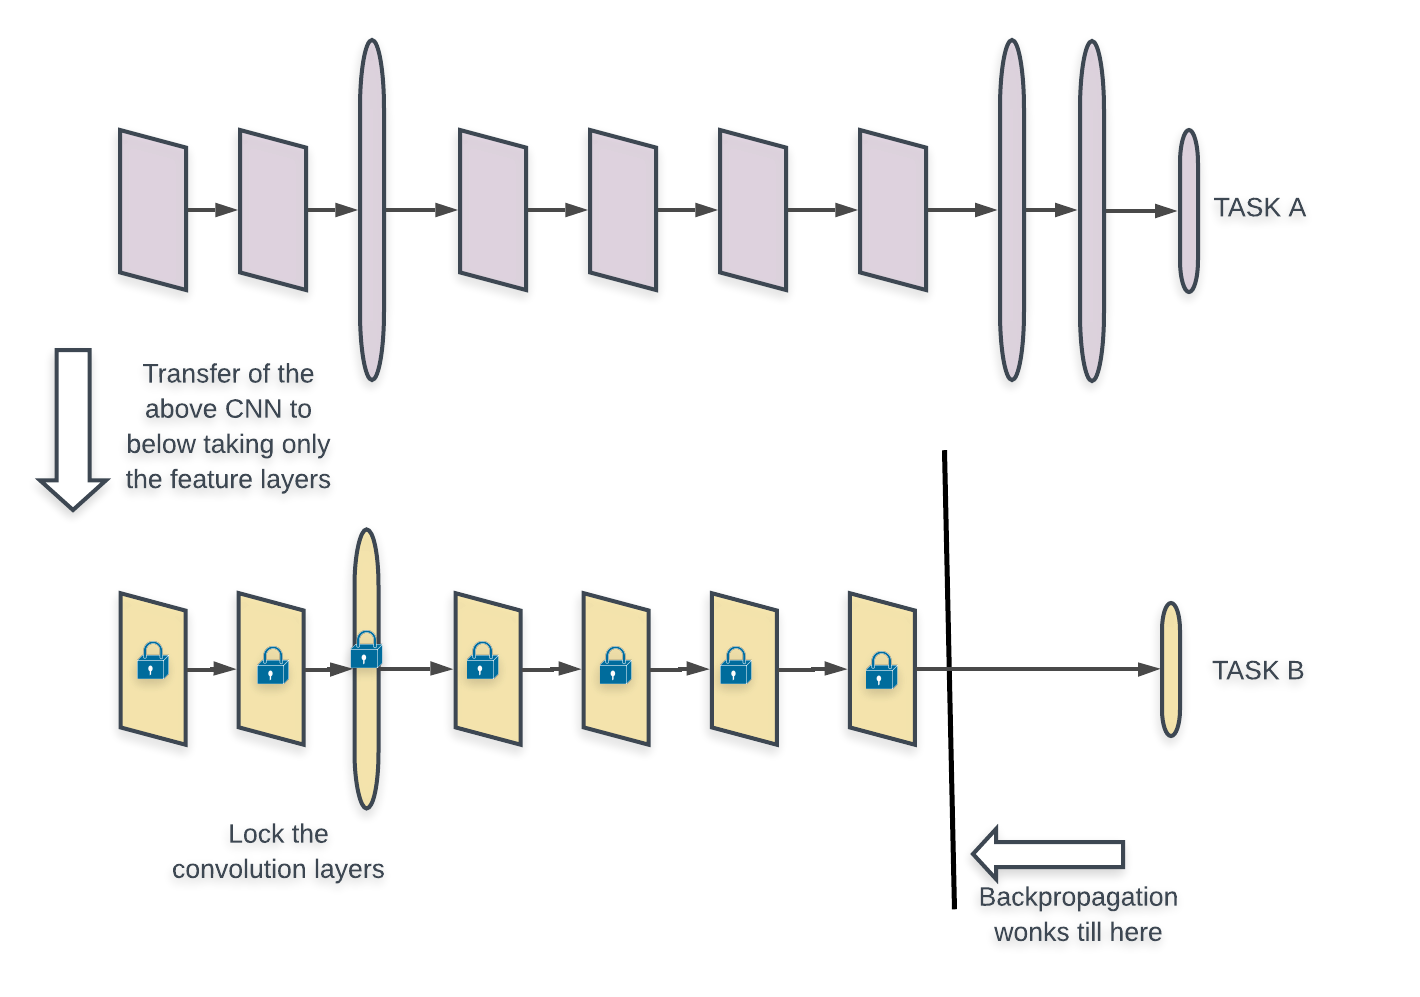
\includegraphics[scale=0.2]{Figures/transfer_learning.png}
\end{center}
\caption{Transfer Learning}
\label{fig:}
\end{figure}

To proceed with this example we will download a pretrained model.

\begin{lstlisting}[caption={chapter6/pytorch-image-classification/src/main.rs}, basicstyle=\small]
wget https://github.com/LaurentMazare/ocaml-torch/releases/download/v0.1-unstable/resnet18.ot
\end{lstlisting}

To be able to do this we will need to load the data set.

\begin{lstlisting}[caption={chapter6/pytorch-image-classification/src/main.rs}, basicstyle=\small]
let dataset = imagenet::load_from_dir(dataset_dir)?;
\end{lstlisting}

Similar to the pretrained network we will need to create the model and load the weights to the model.

\begin{lstlisting}[caption={https://github.com/LaurentMazare/tch-rs/blob/master/examples/transfer-learning/main.rs}, basicstyle=\small]
let mut vs = tch::nn::VarStore::new(tch::Device::Cpu);
let net = resnet::resnet18_no_final_layer(&vs.root());
vs.load(weights)?;
\end{lstlisting}

We will need to store the output of the model in such a way that we are able to create the resulting vectors and tell pytorch that we dont need to store the graph as we are not going to compute the gradients.

\begin{lstlisting}[caption={https://github.com/LaurentMazare/tch-rs/blob/master/examples/transfer-learning/main.rs}, basicstyle=\small]
let train_images = tch::no_grad(|| dataset.train_images.apply_t(&net, false));
let test_images = tch::no_grad(|| dataset.test_images.apply_t(&net, false));
\end{lstlisting}

\subsection{Training}%
We can now append a small linear layer on top of the extracted layers and train only they part of the layer. This way our less data will be used to effectively train only a small part of the net instead of trying to train on the whole model. We create the model and a variable store is used to store the trainable variables.

\begin{lstlisting}[caption={https://github.com/LaurentMazare/tch-rs/blob/master/examples/transfer-learning/main.rs}, basicstyle=\small]
let vs = tch::nn::VarStore::new(tch::Device::Cpu);
let linear = nn::linear(vs.root(), 512, dataset.labels, Default::default());
\end{lstlisting}

Similar to the previous code we can use adam to minimise the cross entropy loss in the classification task. Hence we will need to create an optimizer and iterate on the training dataset. After each epoch the accuracy is computed on the training set and printed.

\begin{lstlisting}[caption={https://github.com/LaurentMazare/tch-rs/blob/master/examples/transfer-learning/main.rs}, basicstyle=\small]
let optimizer = nn::Adam::default().build(&vs, 1e-4)?;
for epoch_idx in 1..1001 {
  let predicted = train_images.apply(&linear);
  let loss = predicted.cross_entropy_for_logits(&dataset.train_labels);
  optimizer.backward_step(&loss);

  let test_accuracy = test_images
    .apply(&linear)
    .accuracy_for_logits(&dataset.test_labels);
  println!("{} {:.2}%", epoch_idx, 100. * f64::from(test_accuracy));
}
\end{lstlisting}

Once the training is done we can save the file using \lstinline{vs.save("model.ot")?;} which can be again reused in a later training cycle when the next batch of images are ready.

\label{sub:Training}
\label{sec:Transfer Learning}

\subsection{Neural Style transfer}%
Neural style transfer is a technique used to generate images in the style of another image. The neural style algorithm takes a content-image and a style image as input and returns the content image transformed in the style of the style image. This is done by creating two distances one for the content and another for the image. A new image is created such that the content distance from the content image and the style distance from the style image is minimized.
% https://towardsdatascience.com/neural-style-transfer-23a3fb4c6a9e
% https://towardsdatascience.com/style-transfer-styling-images-with-convolutional-neural-networks-7d215b58f461

\paragraph{Content Loss}%
To create such a transformed image we need a way to control the amount of content image that ends up in the optimized output image. For this a way to determine the content loss needs to be determined. The main challenge in the content loss is figuring out a way to extract only the content features of an image, and not the style of the image. The solution to this as per the Artistic Style paper\cite[]{CV:2} is that using the feature maps of the different convolutional layers should solve this problem. Trained convnets learn to represent different parts of the image, the initial layers capture the rough, underlying pattern and the final layers capture the distinct features. Its the intermediate layers that capture the spatial characteristics of the image which is what is needed here.

Thus in this case the content loss is calculated by just computing the mean-square error on some of the upper layers. This error helps in ensuring that the extracted images happen at the same on-screen places between the content and current images.

\begin{lstlisting}[caption={https://github.com/LaurentMazare/tch-rs/blob/master/examples/neural-style-transfer/main.rs}, basicstyle=\small]
let content_loss: Tensor = CONTENT_INDEXES
	.iter()
        .map(|&i| input_layers[i].mse_loss(&content_layers[i], 1))
        .sum();
\end{lstlisting}

\label{par:content_loss}
\paragraph{Style loss}%
The style loss is responsible for incorporating the style of image in the final image. According to the paper the style of an image can be encoded using a gram matrix of the image. The gram matrix is made by computing the dot product of the flattened style features and themselves.

\begin{lstlisting}[caption={https://github.com/LaurentMazare/tch-rs/blob/master/examples/neural-style-transfer/main.rs}, basicstyle=\small]
fn gram_matrix(m: &Tensor) -> Tensor {
  let (a, b, c, d) = m.size4().unwrap();
  let m = m.view(&[a * b, c * d]);
  let g = m.matmul(&m.tr());
  g / (a * b * c * d)
}

fn style_loss(m1: &Tensor, m2: &Tensor) -> Tensor {
  gram_matrix(m1).mse_loss(&gram_matrix(m2), 1)
}

let style_loss: Tensor = STYLE_INDEXES
  .iter()
  .map(|&i| style_loss(&input_layers[i], &style_layers[i]))
  .sum();
\end{lstlisting}

Observe that the style of an image is not dependent on the pixel values but the relationship between the pixel values. The gram matrix delocalises all the information of the style image, such as texture, shape and weights and then the dot product is taken. This results in features that co-occur more get greater weightage and features that do not have similarity across the style image do not get weightage. 
\label{par:style_loss}

Now that we have the basic idea on how style transfer works, lets look at the full implementation. To be able to do neural style transfer, we will need to load the content image and the style image. These will need to be torch tensors and hence we can use the imagenet module from \lstinline{tch::vision} to load the images.

\begin{lstlisting}[caption={https://github.com/LaurentMazare/tch-rs/blob/master/examples/neural-style-transfer/main.rs}, basicstyle=\small]
let style_img = imagenet::load_image(style_img)?
  .unsqueeze(0)
  .to_device(device);
let content_img = imagenet::load_image(content_img)?
  .unsqueeze(0)
  .to_device(device);
\end{lstlisting}

We will also need to load a pretrained model. We can use a 19 layer VGG network like the one used in the paper. This is another hyper parameter that you can experiment with and see if there can be another model that would provide a better feature for the content image. Download the model by going to this link or using your favorite download command.

\begin{lstlisting}[caption={}, basicstyle=\small]
$ wget https://github.com/LaurentMazare/ocaml-torch/releases/download/v0.1-unstable/vgg16.ot
\end{lstlisting}

This VGG model consists of two Sequential child modules: features (containing the convolution and pooling layers), and the classifier (containing the fully connected layers). To be able to capture the content from the image we will need to use the features layer. We will load the weights from the model and freeze the model.

\begin{lstlisting}[caption={https://github.com/LaurentMazare/tch-rs/blob/master/examples/neural-style-transfer/main.rs}, basicstyle=\small]
let mut net_vs = tch::nn::VarStore::new(device);
let net = vgg::vgg16(&net_vs.root(),
                     imagenet::CLASS_COUNT);
net_vs.load(weights)?;
net_vs.freeze();
\end{lstlisting}

We now run the model on the style and content images. These calls returns a vector of the extracted features for each of the model layers.

\begin{lstlisting}[caption={https://github.com/LaurentMazare/tch-rs/blob/master/examples/neural-style-transfer/main.rs}, basicstyle=\small]
let style_layers = net.forward_all_t(
  &style_img, false, Some(max_layer));
let content_layers = net.forward_all_t(
  &content_img, false, Some(max_layer));
\end{lstlisting}

We will use gradient optimization method to optimize an image. For that we create a second variable store to hold this image. The initial values for this image will be by copying the content image. This image will be transformed so that the style is similar to the style image.

\begin{lstlisting}[caption={}, basicstyle=\small]
let vs = nn::VarStore::new(device);
let input_var = vs.root().var_copy("img", &content_img);
\end{lstlisting}

We will now create the optimizer which will be an instance of the use Adam optimization algorithm.

\begin{lstlisting}[caption={}, basicstyle=\small]
let opt = nn::Adam::default().build(&vs, LEARNING_RATE)?;
\end{lstlisting}

Now in the gradient descent loop cycle the content and style losses will need to be computed. They will then be summed together and the aggregate loss will be optimized using the optimizer created above. For every 1000 epochs we can compute the current loss and write the current image to file.

\begin{lstlisting}[caption={}, basicstyle=\small]
for step_idx in 1..(1 + TOTAL_STEPS) {
  let input_layers = net.forward_all_t(
    &input_var, false, Some(max_layer));
  let style_loss: Tensor = STYLE_INDEXES
    .iter()
    .map(
      |&i| style_loss(&input_layers[i], &style_layers[i]))
    .sum();
  let content_loss: Tensor = CONTENT_INDEXES
    .iter()
    .map(
      |&i| input_layers[i].mse_loss(&content_layers[i], 1))
    .sum();
  let loss = style_loss * STYLE_WEIGHT + content_loss;
  opt.backward_step(&loss);
  if step_idx % 1000 == 0 {
    println!("{} {}", step_idx, f64::from(loss));
    imagenet::save_image(&input_var, &format!("out{}.jpg", step_idx))?;
  }
}
\end{lstlisting}

We should be able to run the code now. Keep the \lstinline{TOTAL_STEPS} 5000 or higher so that we have a high number of images and can chose the image that seems the most coherent yet similar to the target style.

\label{sub:neural_style_transfer}

\section{Tensorflow and Face Detection}%
In the previous sections we have mostly worked torch and the corresponding Rust framework \lstinline{tch}. In this section we will be using tensorflow and look at an application for face detection. The challenge is to take an image identify the faces and create a new image with boxes drawn around the faces. As seen in chapter2, just running the inference in tensorflow is easier than training a model and hence we will mostly be working towards model inference in this case.
% https://cetra3.github.io/blog/face-detection-with-tensorflow-rust/

\begin{figure}
\begin{center}
	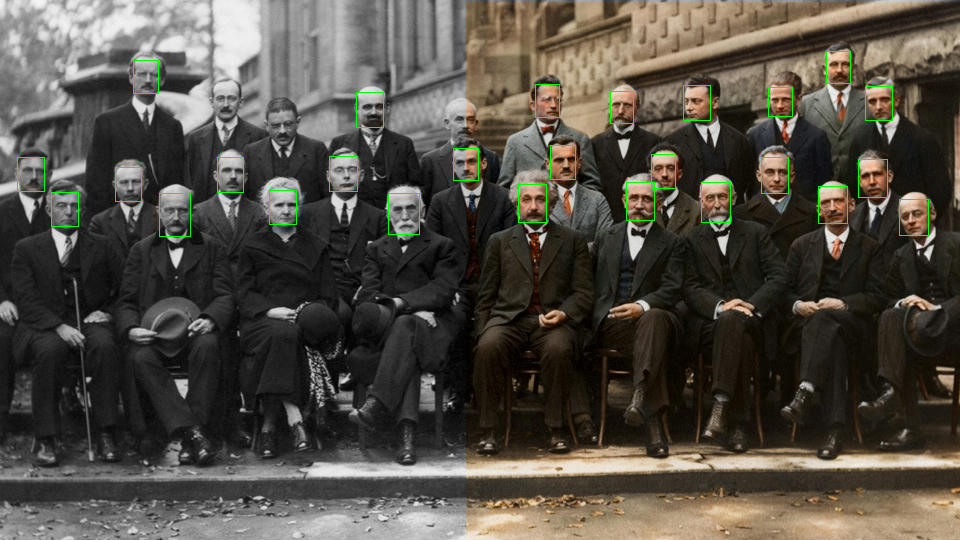
\includegraphics[scale=0.2]{Figures/scientists.jpg}
\end{center}
\caption{Famous Scientists}
%\captionsource{Image Source}{\href{}{http://sannadullaway.com/7xdocsffg0d917t2gqkbqpqyz36qgx}}
\label{fig:}
\end{figure}

Download the following trained model. This model will be used to predict on an image. Figure 5 is the predicted image with the faces boxed\footnote{Original Image Source http://sannadullaway.com/7xdocsffg0d917t2gqkbqpqyz36qgx}.

\begin{lstlisting}[caption={}, basicstyle=\small]
$ wget https://github.com/blaueck/tf-mtcnn/blob/master/mtcnn.pb
\end{lstlisting}

Now lets talk about the dependencies. We will need tensorflow to read the model and make the inferences on an image using the model. We will structopt would be used to parse the command line and make the input output parsing better. Apart from these we will need image and image to read, write and make changes in the image. Hence we should have a \lstinline{Cargo.toml} similar to the one shown below.

\begin{lstlisting}[caption={chapter6/face-detection-tf/src/main.rs}, basicstyle=\small]
[package]
name = "face-detection-tf"
version = "0.1.0"
authors = ["put your name here."]
edition = "2018"

[dependencies]
tensorflow = "0.13.0"
structopt = "0.2.15"
image = "0.21.1"
imageproc = "0.18.0"
\end{lstlisting}

We can now start with defining the command line. Our app can have the image file name as one of the inputs and an output file name as the file that would need to be created with the faces identified.

\begin{lstlisting}[caption={chapter6/face-detection-tf/src/main.rs}, basicstyle=\small]
use std::path::PathBuf;
use structopt::StructOpt;

#[derive(Debug, StructOpt)]
#[structopt(name = "face-detection-tf", about = "Face Identification")]
struct Opt {
    #[structopt(short = "i", long = "input", parse(from_os_str))]
    input: PathBuf,

    #[structopt(short = "o", long = "output", parse(from_os_str))]
    output: PathBuf
}
\end{lstlisting}

Creating the above \lstinline{StructOpt} struct means that when we plugin \lstinline{let opt = Opt::from_args();} in the main function, we will be able to pass command line arguments in the format \lstinline{./face-detection-tf -i inputfilename.jpg -o outputfilename.jpg} or pass \lstinline{--input} and \lstinline{--output} as the command line arguments. To run this check if the command line arguments run now, we can put the following lines in the main function of the code and check if the command lines are being parsed correctly.

\begin{lstlisting}[caption={chapter6/face-detection-tf/src/main.rs}, basicstyle=\small]
use std::error::Error;
fn main() -> Result<(), Box<dyn Error>> {
    let opt = Opt::from_args();
    // since this is plumbing we will take
    // care that we dont move over ownership of the
    // opt objects using to_owned
    println!("{:?}", (opt.input.to_owned(), opt.output.to_owned()));
    Ok(())
}
\end{lstlisting}

Now running cargo run should give us the correct outputs.

\begin{lstlisting}[caption={chapter6/face-detection-tf/src/main.rs}, basicstyle=\small]
$ cargo run -- -i rustfest.jpg -o out.jpg
   Compiling face-detection-tf v0.1.0 (path to face-detection-tf)

    Finished dev [unoptimized + debuginfo] target(s) in 28.24s
     Running `target/debug/face-detection-tf -i rustfest.jpg -o out.jpg`
("rustfest.jpg", "out.jpg")
\end{lstlisting}

We can now see if we are able to load the model. We will first load the model as a byte array and then we will try to infer the graph from the byte array. If the model file is corrupted this should given an error in this case.

\begin{lstlisting}[caption={chapter6/face-detection-tf/src/main.rs}, basicstyle=\small]
use tensorflow::Graph;
use tensorflow::ImportGraphDefOptions;
use tensorflow::{Session, SessionOptions, SessionRunArgs, Tensor};

fn main() -> Result<(), Box<dyn Error>> {
  ... prev code ...
  let model = include_bytes!("../mtcnn.pb");
  let mut graph = Graph::new();
  graph.import_graph_def(&*model, &ImportGraphDefOptions::new())?;
  .. rem code ...
\end{lstlisting}

If the graph is loaded successfully, we should be able to create a session with this graph.

\begin{lstlisting}[caption={chapter6/face-detection-tf/src/main.rs}, basicstyle=\small]
let session = Session::new(&SessionOptions::new(), &graph)?;
\end{lstlisting}

Now if we check the model from which the graph is created, we can see that there are some variables that needs to be set before running the model as seen in this line for the model \href{https://github.com/blaueck/tf-mtcnn/blob/master/mtcnn.py#L9}{https://github.com/blaueck/tf-mtcnn/blob/master/mtcnn.py\#L9}. These variables are \lstinline{min_size}, \lstinline{factor} and \lstinline{thresholds}. We will need to assign those variables in our session so before running the session. The values that are assigned below are the same as had been used for the model but you play around with these values and see if there are better alternatives.

\begin{lstlisting}[caption={chapter6/face-detection-tf/src/main.rs}, basicstyle=\small]
let min_size = Tensor::new(
	&[]).with_values(&[40f32])?;
let thresholds = Tensor::new(&[3]).with_values(
	&[0.6f32, 0.7f32, 0.7f32])?;
let factor = Tensor::new(&[]).with_values(&[0.709f32])?;

let mut args = SessionRunArgs::new();

//Load our parameters for the model
args.add_feed(
	&graph.operation_by_name_required("min_size")?,
	0, &min_size);
args.add_feed(
	&graph.operation_by_name_required("thresholds")?,
	0, &thresholds);
args.add_feed(
	&graph.operation_by_name_required("factor")?,
	0, &factor);
\end{lstlisting}

One other variable that needs to be passed and the most important one that will enable the graph to make facepredictions is the input image tensor. So we will open the input image using the image crate. Once the image is opened we will read the values and store in a tensor in BGR format\footnote{We will need to store in BGR instead of RGB because the model was created to support opencv. Go to this link for further information https://stackoverflow.com/a/33787594/5417164}.

\begin{lstlisting}[caption={chapter6/face-detection-tf/src/main.rs}, basicstyle=\small]
fn get_input_image_tensor(opt: &Opt) -> Result<Tensor<f32>, Box<dyn Error>> {
  let input_image = image::open(&opt.input)?;

  let mut flattened: Vec<f32> = Vec::new();
  for (_x, _y, rgb) in input_image.pixels() {
    flattened.push(rgb[2] as f32);
    flattened.push(rgb[1] as f32);
    flattened.push(rgb[0] as f32);
  }
  let input = Tensor::new(
    &[input_image.height() as u64, input_image.width() as u64, 3])
    .with_values(&flattened)?;
  Ok(input)
}
\end{lstlisting}

So now similar to listing32, we should be able to load the image to the graph as the input.

\begin{lstlisting}[caption={chapter6/face-detection-tf/src/main.rs}, basicstyle=\small]
let input = get_input_image_tensor(&opt)?;
args.add_feed(&graph.operation_by_name_required("input")?, 0, &input);
\end{lstlisting}

Now that the inputs are taken care of, we need to create endpoints for the outputs. This will enable us to fetch the results when the session is run.

\begin{lstlisting}[caption={chapter6/face-detection-tf/src/main.rs}, basicstyle=\small]
let bbox = args.request_fetch(&graph.operation_by_name_required("box")?, 0);
let prob = args.request_fetch(&graph.operation_by_name_required("prob")?, 0);

session.run(&mut args)?;

let bbox_res: Tensor<f32> = args.fetch(bbox)?;
let prob_res: Tensor<f32> = args.fetch(prob)?;
\end{lstlisting}

The above code should output \lstinline{bbox_res} of dimensions [120, 4] and \lstinline{prob_res} of dimensions [120].

Now that we will need to parse the outputs and store in a struct so that we are able to draw the bounding boxes. For this reason we will create a BBox struct so that we are able to store the outputs.

\begin{lstlisting}[caption={chapter6/face-detection-tf/src/main.rs}, basicstyle=\small]
#[derive(Copy, Clone, Debug)]
pub struct BBox {
  pub x1: f32,
  pub y1: f32,
  pub x2: f32,
  pub y2: f32,
  pub prob: f32,
}
\end{lstlisting}

We should now be able to store the results as a \lstinline{Vec<BBox>}.

\begin{lstlisting}[caption={chapter6/face-detection-tf/src/main.rs}, basicstyle=\small]
let bboxes: Vec<_> = bbox_res
  .chunks_exact(4)
  .zip(prob_res.iter()) // combine with the probability outputs
  .map(|(bbox, &prob)| BBox {
    y1: bbox[0], x1: bbox[1],
    y2: bbox[2], x2: bbox[3],
    prob,
  }).collect();
\end{lstlisting}

We should now be able to draw the rectangles around the faces for the input figure. For that we will create a new image, called \lstinline{output_image} and which of course should be mutable, with the input image and for all the bboxes we will draw rectangles at \lstinline{x1} and \lstinline{y1} with sizes \lstinline{(bbox.x2 - bbox.x1)} and \lstinline{(bbox.y2 - bbox.y1)}. Once the images have been updated with rectangles we can save the changed image.

\begin{lstlisting}[caption={chapter6/face-detection-tf/src/main.rs}, basicstyle=\small]
let mut output_image = image::open(&opt.input)?;

for bbox in bboxes {
  let rect = Rect::at(bbox.x1 as i32, bbox.y1 as i32)
    .of_size((bbox.x2 - bbox.x1) as u32, (bbox.y2 - bbox.y1) as u32);
  draw_hollow_rect_mut(&mut output_image, rect, LINE_COLOUR);
}
output_image.save(&opt.output)?;
\end{lstlisting}

We should now be able to see the output file in folder with boxes drawn around the faces.

\label{sec:tensorflow_and_face_detection}


\section{Conclusion}%

This chapter introduced to different interesting applications in Computer Vision. The chapter started with image classification and how to build an image classifier using tch library which allows easy usage of the pytorch deep learning library. Then the chapter went on with using pretrained networks for image classification when the number of samples in the data set are small. The next application for discussion was Neural Style transfer and an application was created that took in a content image and a style image and transformed the content image in the style of the style image. The next application in the chapter how Generative Neural Networks work and creating a fake facial creator app using the tch library. After mostly working in the tch library, the chapter also included an application in identifying faces in an image using the tensorflow library.

In the next chapter, you will learn about other different needs in machine learning such as statistical analysis in Rust and recommender systems.
\label{sec:conclusion}

\printbibliography
\nocite{*}
\end{document}
